%!TEX root = ../dissertation.tex
\chapter{Co-authored publications using Orthograph}
\label{app:papers-using-orthograph}

% if draft
\ifdraft{%
	\section{\citet{Johnson2018}, submitted to PNAS}
	\emptypages{30} % Johnson 2018
	\section{\citet{Gillung2018}}
	\emptypages{13} % Gillung 2018
	\section{\citet{Peters2017}}
	\emptypages{6} % Peters 2017
	\section{\citet{Dowling2017}}
	\emptypages{10} % Dowling 2017
	\section{\citet{Bank2017}}
	\emptypages{14} % Bank 2017
	\section{\citet{Pauli2016}}
	\emptypages{10} % Pauli 2016
	\section{\citet{Mayer2016}}
	\emptypages{12} % Mayer 2016
}%
% if not draft
{%
%\addtocounter{section}{1}
%\addcontentsline{toc}{section}{A.\arabic{section}\quad \citet{Johnson2018}: Phylogenomics and the evolution of hemipteroid insects (submitted to PNAS)}
\includepdf[addtotoc={1,section,1,\citet{Johnson2018}: Phylogenomics and the evolution of hemipteroid insects,app:Johnson2018},pages=-30]{appendix/A/Johnson2018} % range without endpoints: from first to last
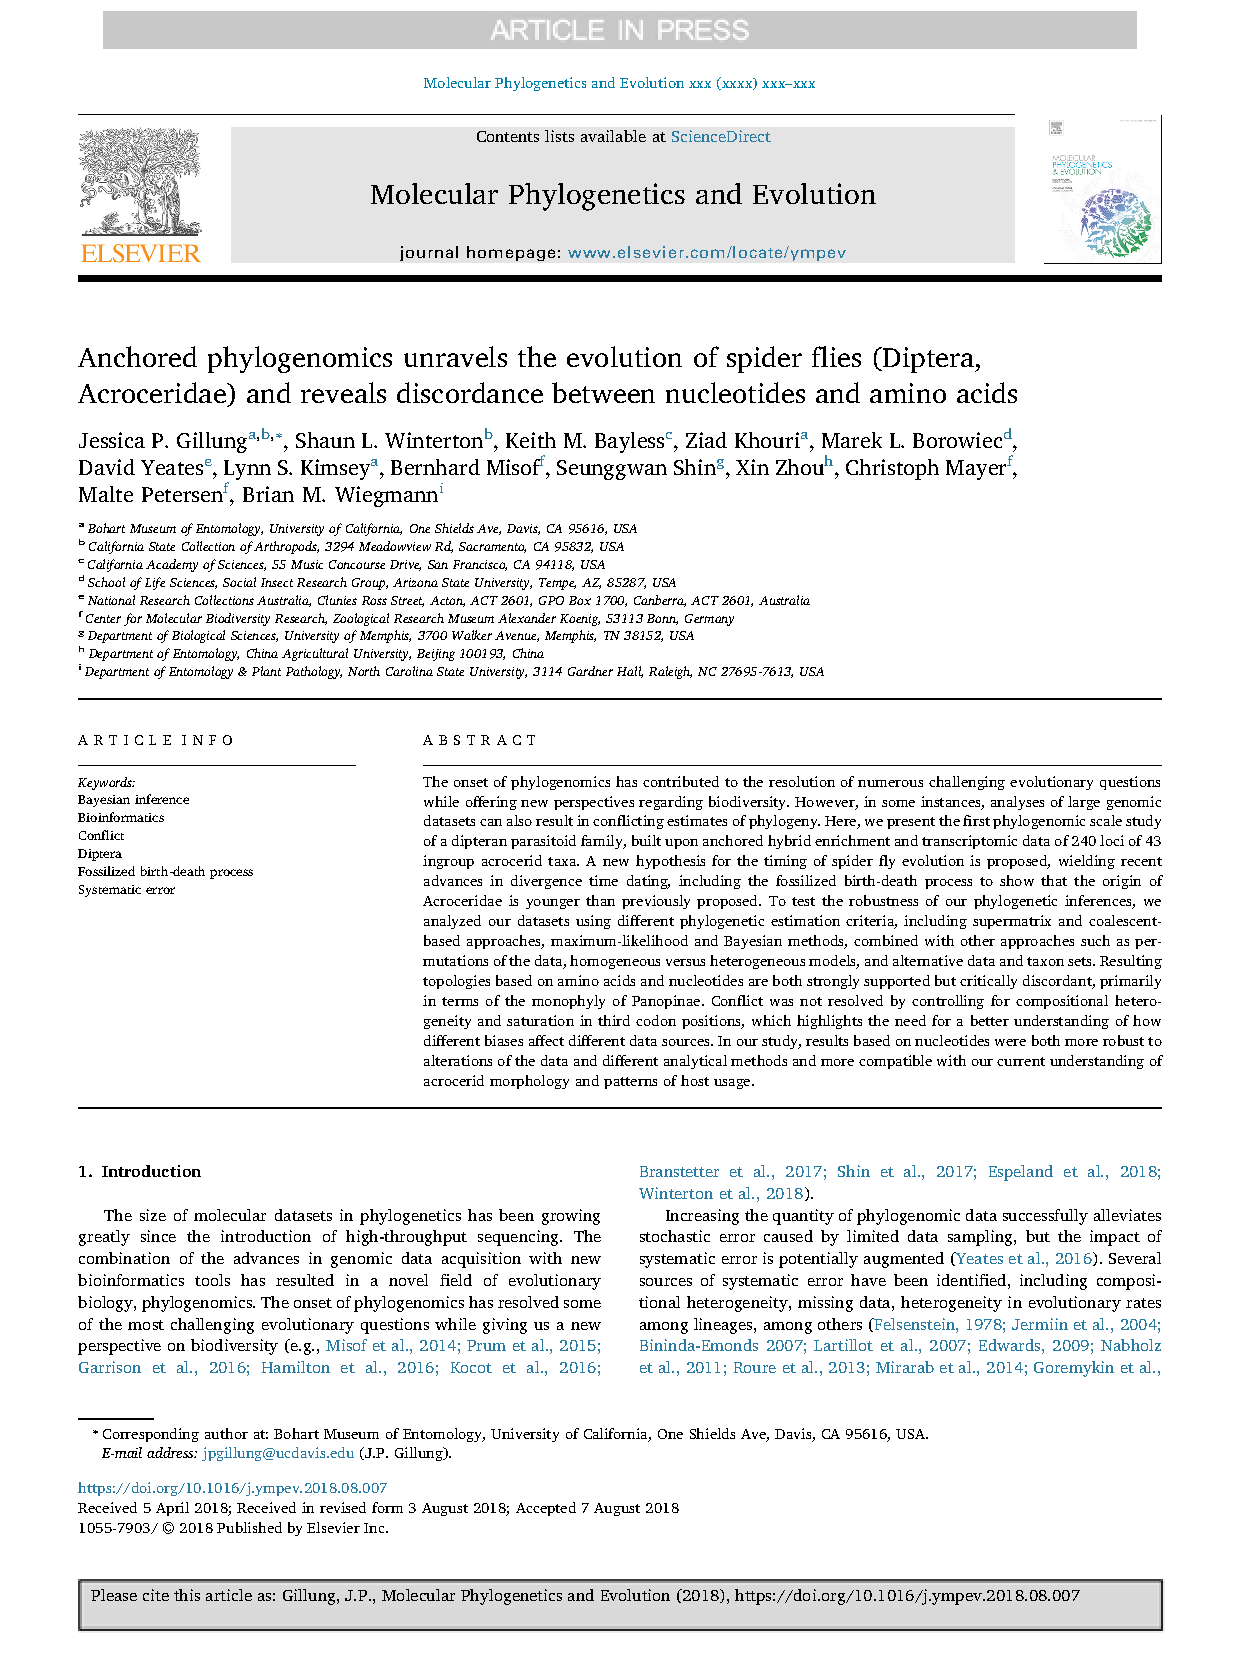
\includepdf[addtotoc={1,section,1,\citet{Gillung2018}: Anchored phylogenomics unravels the evolution of spider flies (Acroceridae) and reveals discordance between nucleotides and amino acids,app:Gillung2018},pages=-]{appendix/A/Gillung2018} % range without endpoints: from first to last
\includepdf[addtotoc={1,section,1,\citet{Peters2017}: Evolutionary history of the Hymenoptera,app:Peters2017},pages=-]{appendix/A/Peters2017} % range without endpoints: from first to last
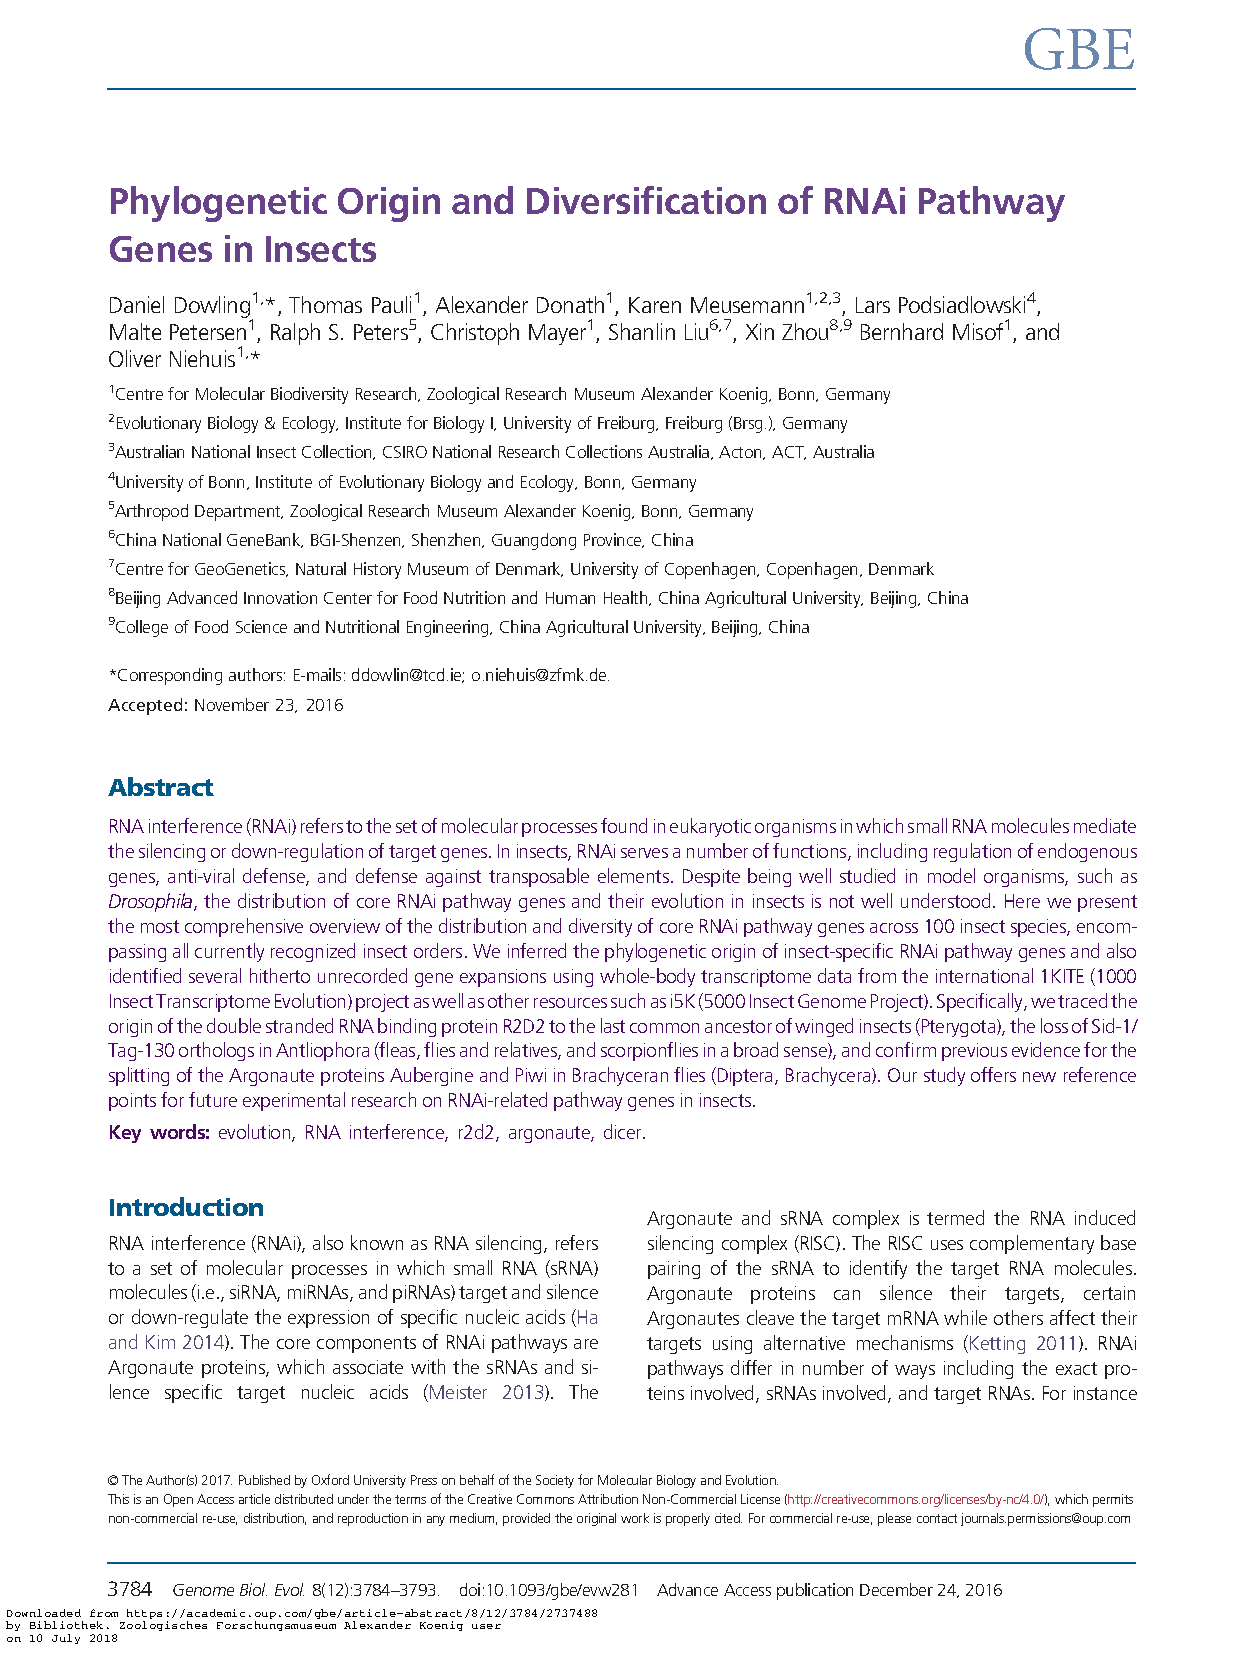
\includepdf[addtotoc={1,section,1,\citet{Dowling2017}: Phylogenetic origin and diversification of RNAi pathway genes in insects,app:Dowling2017},pages=-]{appendix/A/Dowling2017}
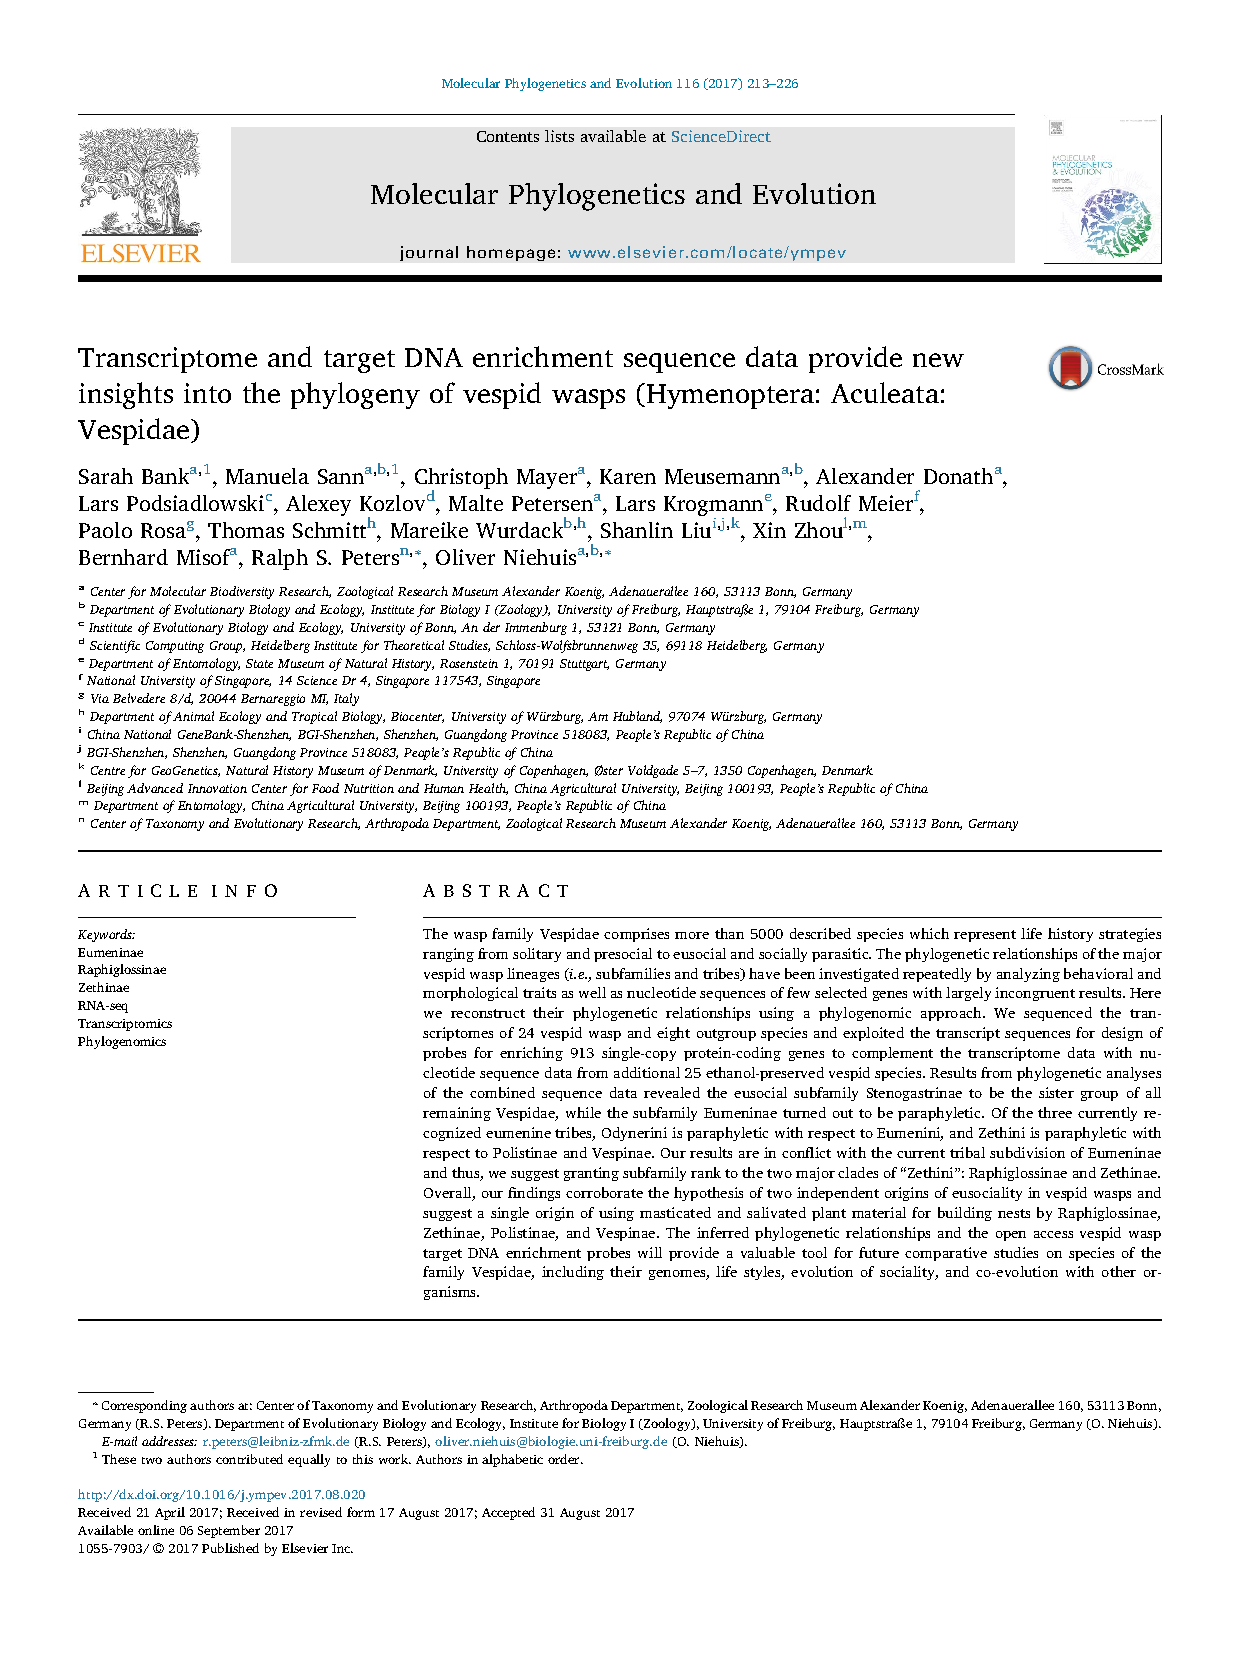
\includepdf[addtotoc={1,section,1,\citet{Bank2017}: New insights into the phylogeny of vespid wasps (Hymenoptera: Aculeata: Vespidae),app:Bank2017},pages=-]{appendix/A/Bank2017}
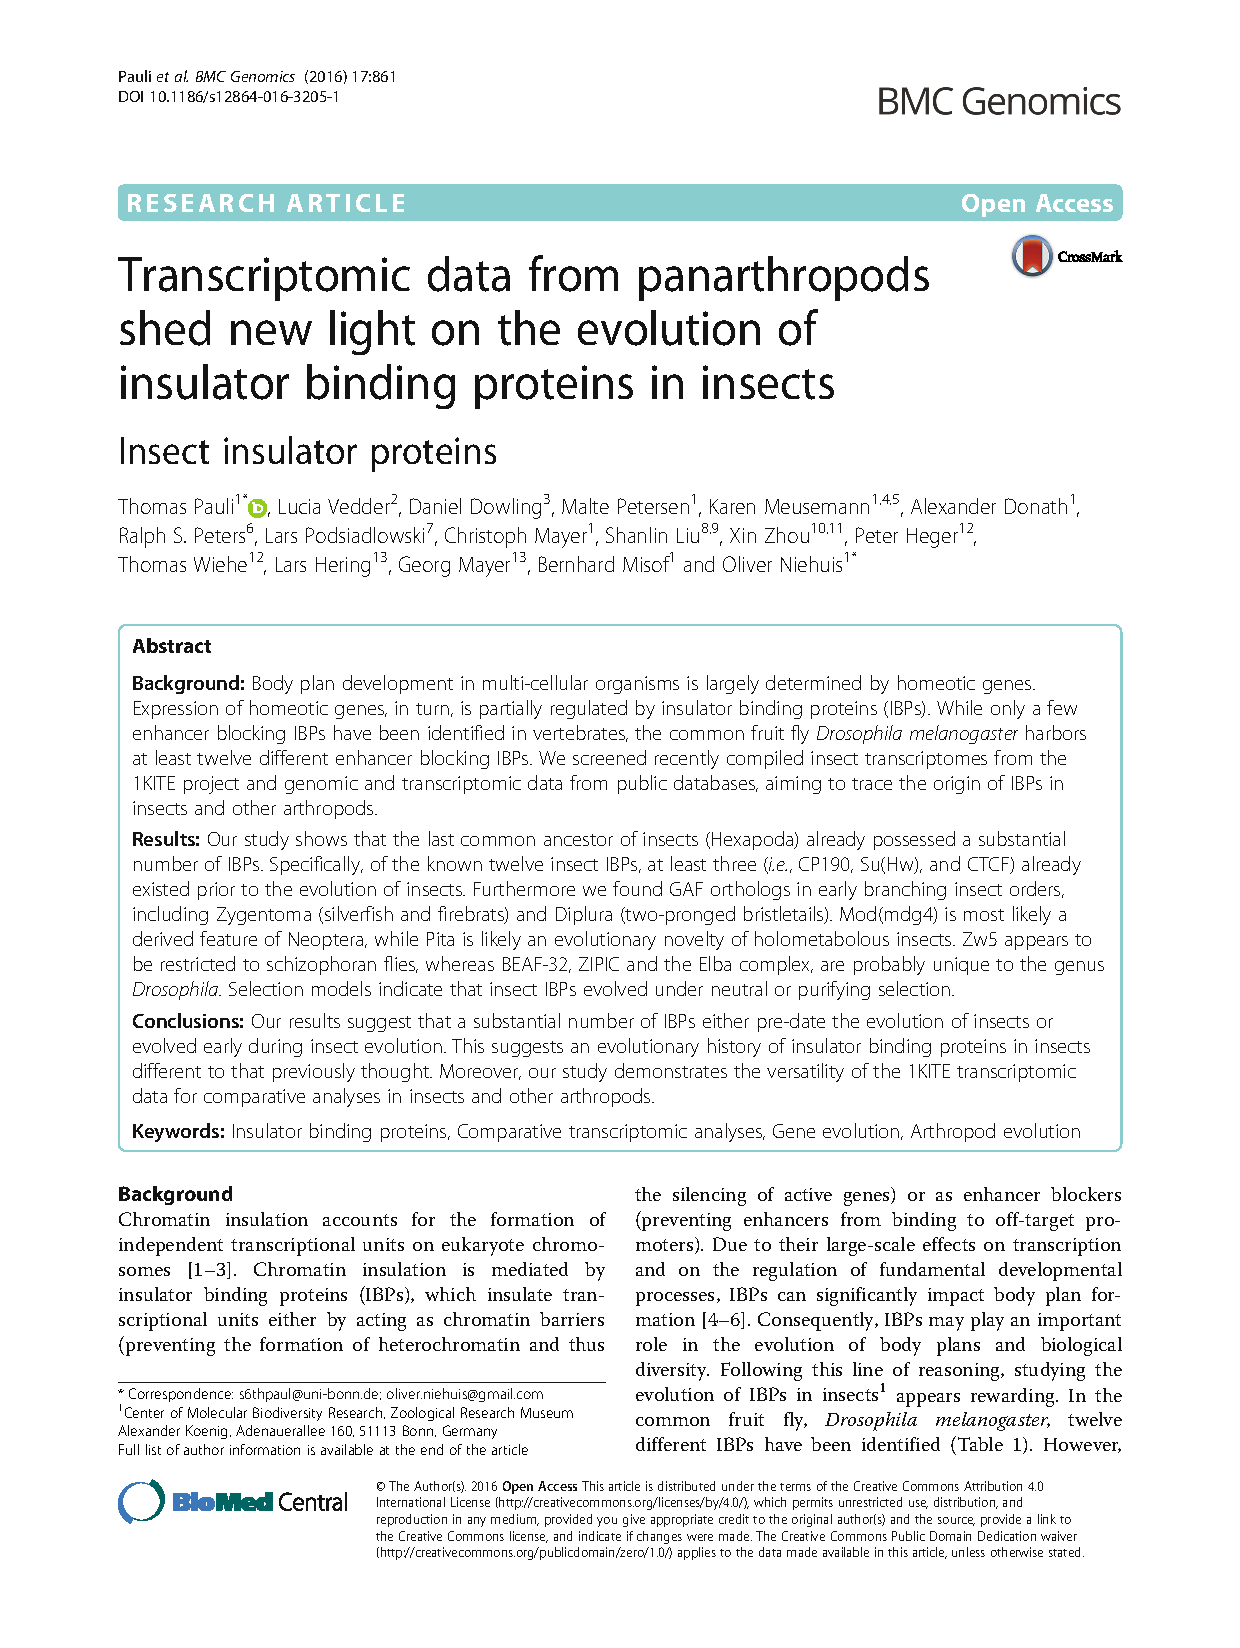
\includepdf[addtotoc={1,section,1,\citet{Pauli2016}: New insights on the evolution of insulator binding proteins in insects ,app:Pauli2016},pages=-]{appendix/A/Pauli2016}
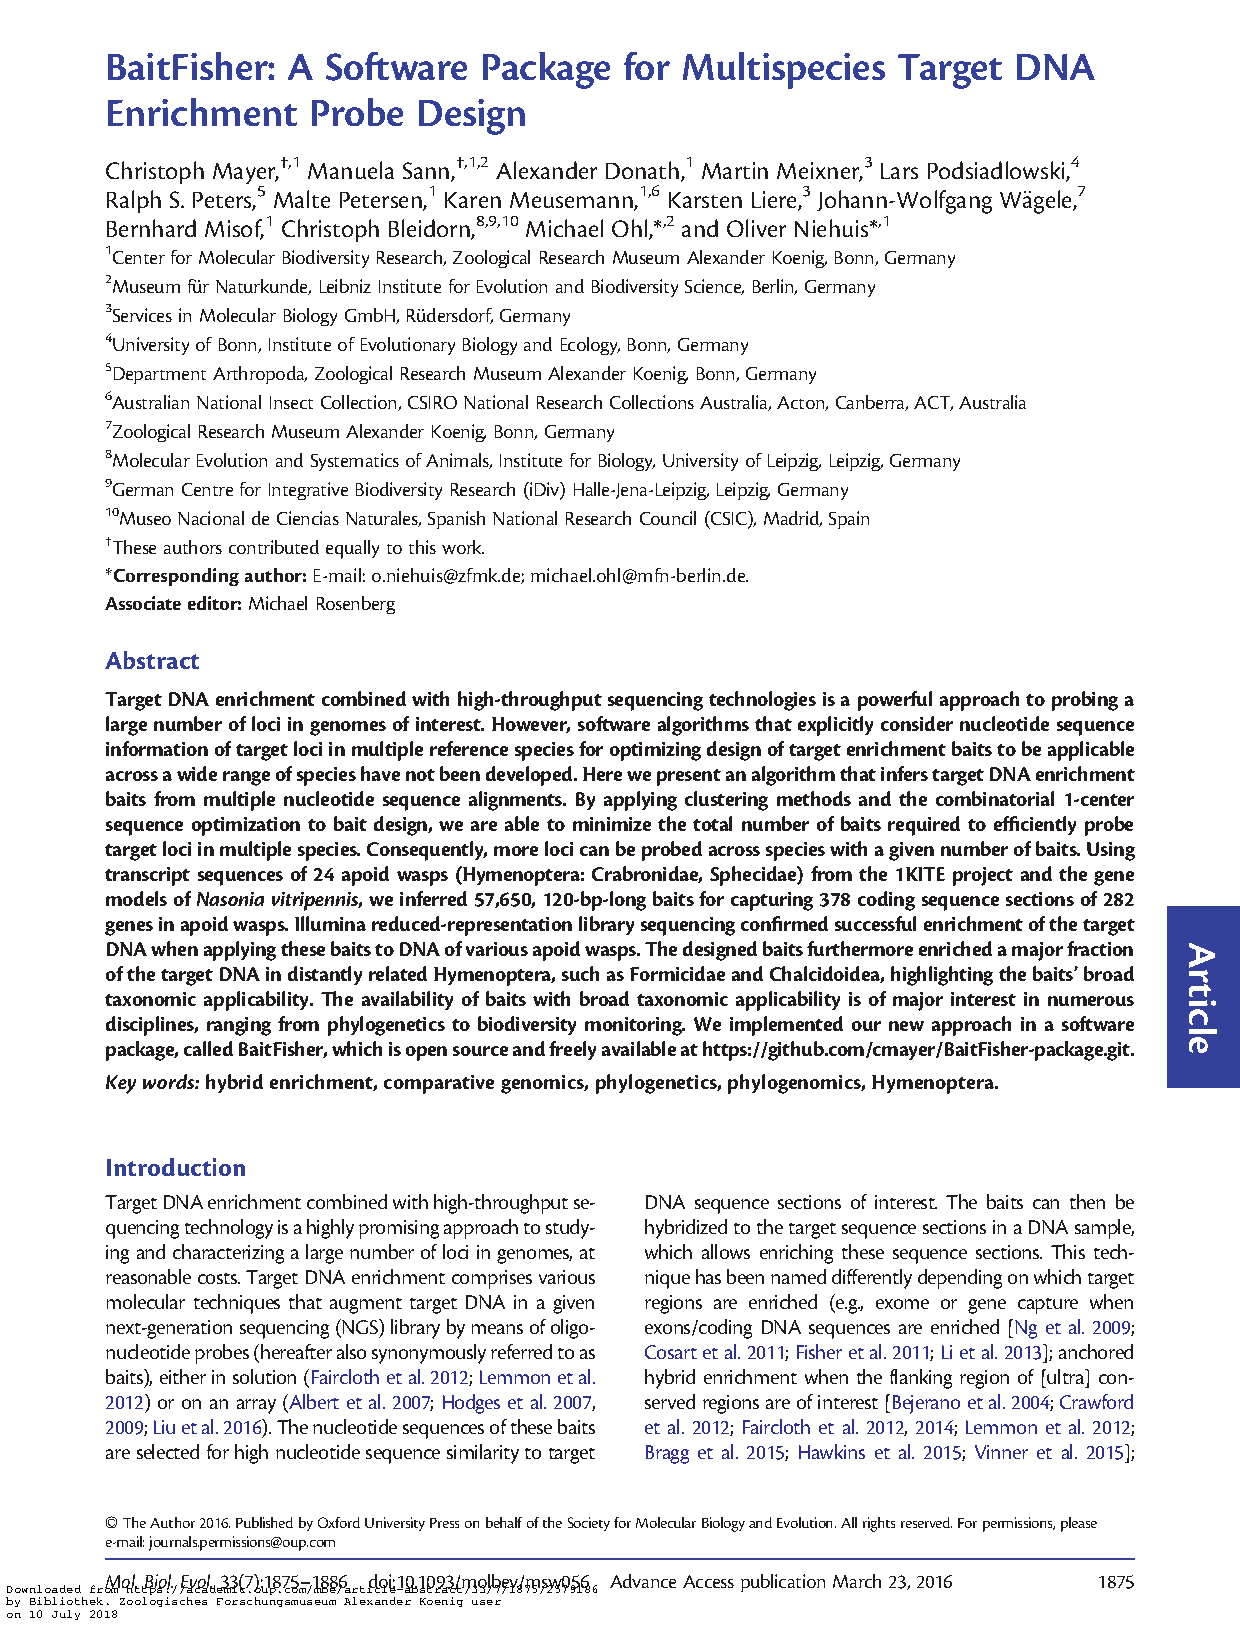
\includepdf[addtotoc={1,section,1,\citet{Mayer2016}: BaitFisher: A software package for multispecies target DNA enrichment probe design ,app:Mayer2016},pages=-]{appendix/A/Mayer2016}
}
